% In your document preamble: \usepackage{booktabs}, \usepackage{hyperref}, \usepackage{longtable}, \usepackage{caption}
\scriptsize
\setlength{\tabcolsep}{3pt}
\begin{longtable}{llllrr@{\hspace{0.8cm}}llllrr}
\captionsetup{labelformat=empty}
\caption{\textbf{SI Table S3. Data for Isomerase Receptors}}
\label{tab:st3} \\
\toprule
apo\_pdb & holo\_pdb & apo\_bmrb & holo\_bmrb & F1 & MCC & apo\_pdb & holo\_pdb & apo\_bmrb & holo\_bmrb & F1 & MCC \\
\midrule
\endfirsthead
\caption[]{(continued)} \\
\toprule
apo\_pdb & holo\_pdb & apo\_bmrb & holo\_bmrb & F1 & MCC & apo\_pdb & holo\_pdb & apo\_bmrb & holo\_bmrb & F1 & MCC \\
\midrule
\endhead
\bottomrule
\endfoot
\bottomrule
\endlastfoot
 & \href{https://www.rcsb.org/structure/2MS4}{2MS4} & \href{https://bmrb.io/data_library/summary/index.php?bmrbId=2208}{2208} & \href{https://bmrb.io/data_library/summary/index.php?bmrbId=25104}{25104} & 0.29 & 0.29 &  & \href{https://www.rcsb.org/structure/7ZEY}{7ZEY} & \href{https://bmrb.io/data_library/summary/index.php?bmrbId=16983}{16983} & \href{https://bmrb.io/data_library/summary/index.php?bmrbId=34727}{34727} & 0.48 & 0.18 \\
 & \href{https://www.rcsb.org/structure/8SG2}{8SG2} & \href{https://bmrb.io/data_library/summary/index.php?bmrbId=27579}{27579} & \href{https://bmrb.io/data_library/summary/index.php?bmrbId=31080}{31080} & 0.44 & 0.23 &  & \href{https://www.rcsb.org/structure/2RSE}{2RSE} & \href{https://bmrb.io/data_library/summary/index.php?bmrbId=50325}{50325} & \href{https://bmrb.io/data_library/summary/index.php?bmrbId=11471}{11471} & 0.05 & -0.02 \\
 & \href{https://www.rcsb.org/structure/7ZEY}{7ZEY} & \href{https://bmrb.io/data_library/summary/index.php?bmrbId=34724}{34724} & \href{https://bmrb.io/data_library/summary/index.php?bmrbId=34727}{34727} & 0.36 & 0.22 &  & \href{https://www.rcsb.org/structure/2RSE}{2RSE} & \href{https://bmrb.io/data_library/summary/index.php?bmrbId=16931}{16931} & \href{https://bmrb.io/data_library/summary/index.php?bmrbId=11471}{11471} & 0.00 & -0.16 \\
\end{longtable}

\begin{figure}[htbp]
\centering
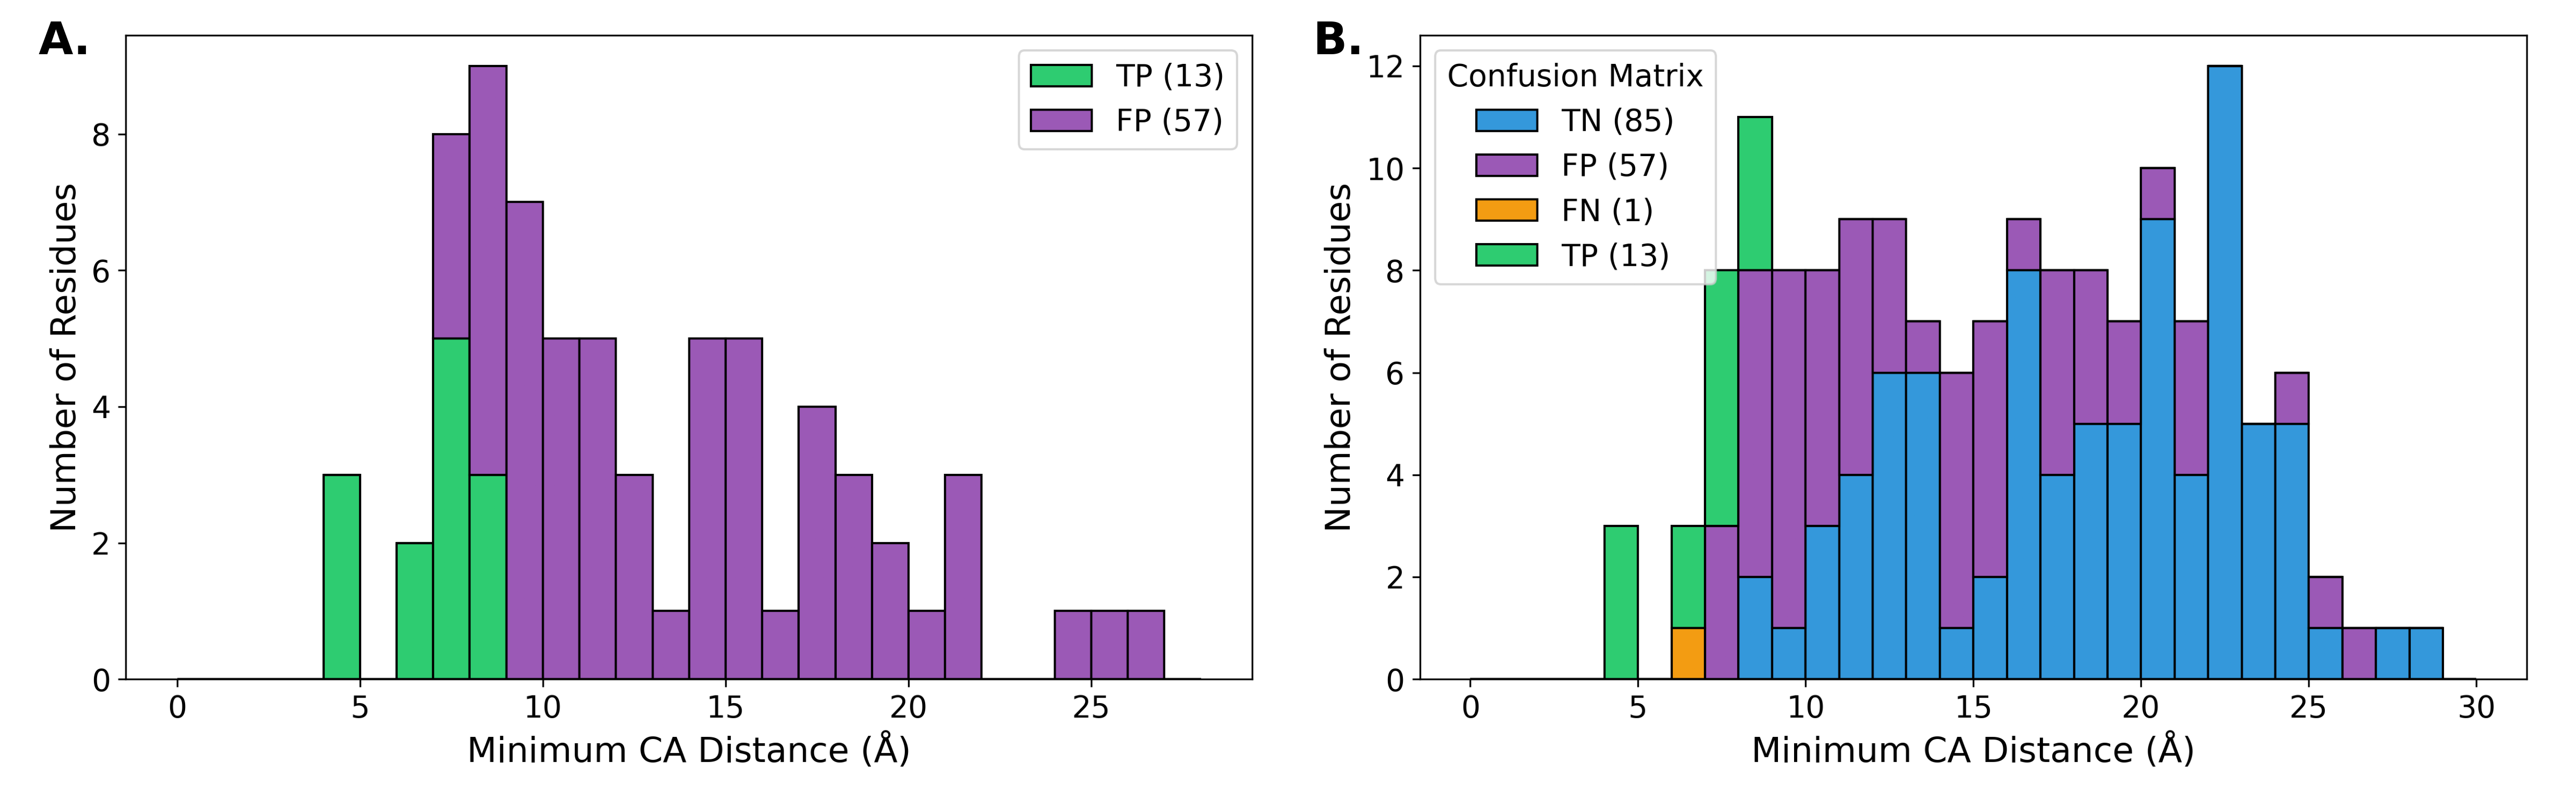
\includegraphics[width=\linewidth]{SF2_isomerases.png}
\captionsetup{labelformat=empty}
\caption{\textbf{SI Fig. S2. Confusion Matrix Histograms for Isomerase Receptors}}
\label{fig:sf2_isomerases}
\end{figure}
